\chapter{Theoretical Background}

This chapter provides a short introduction into Josephson junctions and their role in SQUIDs, which will be the main focus of this thesis. We start with a brief overview on macroscopic quantum phenomena such as the Josephson effect and explain the general working principle of superconductor-isolator-superconductor (SIS) tunnel contacts, followed by a summary of their basic properties . They form the theoretical framework to describe SQUIDs, which are developed in this group and optimized within the scope of this thesis. Lastly, we will take a closer look into their resonance behavior and investigate different solution approaches. 

\section{Josephson junctions}
%Die nach \textit{Brain D. Josephson} benannten \textit{Josephson-Kontakte} (engl. \textit{Josephson junctions}) bestehen aus zwei identischen Supraleitern, die schwach miteinander gekoppelt sind. Im Falle der in dieser Arbeitsgruppe hergestellten Kontakte wird eine solche Kopplung durch eine wenige \r{A}ngström dünne Isolationsschicht zwischen den supraleitenden Elektroden realisiert. Aufgrund dessen werden diese auch SIS (Supraleiter-Isolator-Supraleiter) Kontakte genannt. Die so entstehende Dreischichtstruktur besteht typischerweise aus Nb/Al-Al$O_x$/Nb, wobei das Niob für die Supraleiter verwendet wird und die Isoationsschicht durch das Aluminiumoxid gegeben ist. Ein schematischer Aufbau ist in Abb. ? dargestellt. 
%Wird der Kontakt nun bei sehr kalten Temperaturen ($\leq \qty{4}{\kelvin}$) gehalten und an eine Stromquelle angeschlossen, ist entgegen der Erwartungen ein Suprastrom messbar.

The \textit{Josephson junctions} named after Brian D. Josephson consist of two identical superconductors weakly coupled to each other. In the case of the junctions produced in this working group, such coupling is realized through a few nm thin insulating layer between the superconducting electrodes. Consequently, they are referred to as SIS (Superconductor-Insulator-Superconductor) junctions. The resulting trilayer structure typically consists of Nb/Al-Al$\mathrm{O}_x$/Nb, with niobium being used for the superconductors and the insulating layer being provided by the aluminum oxide. A schematic structure is shown in figure \ref{abb:fig:JJschem}. When the junction is maintained at very cold temperatures ($\leq \qty{4}{\kelvin}$) and connected to a current source a supercurrent is measurable.

\figurecenter {b!}
{width=\textwidth}
{../Figures/jj_schematic}
%{7.8cm}
{0cm}
{Schematic of a Josephson (SIS) junction. Both superconducting electrodes $\textbf{\textit{S}}_\textbf{1}$ and $\textbf{\textit{S}}_\textbf{2}$ are weakly coupled with each other through a thin tunnel barrier \textbf{\textit{I}}. The blue circles 1 and 2 mark the threshold between superconductor and insulator.}
{fig:JJschem}


%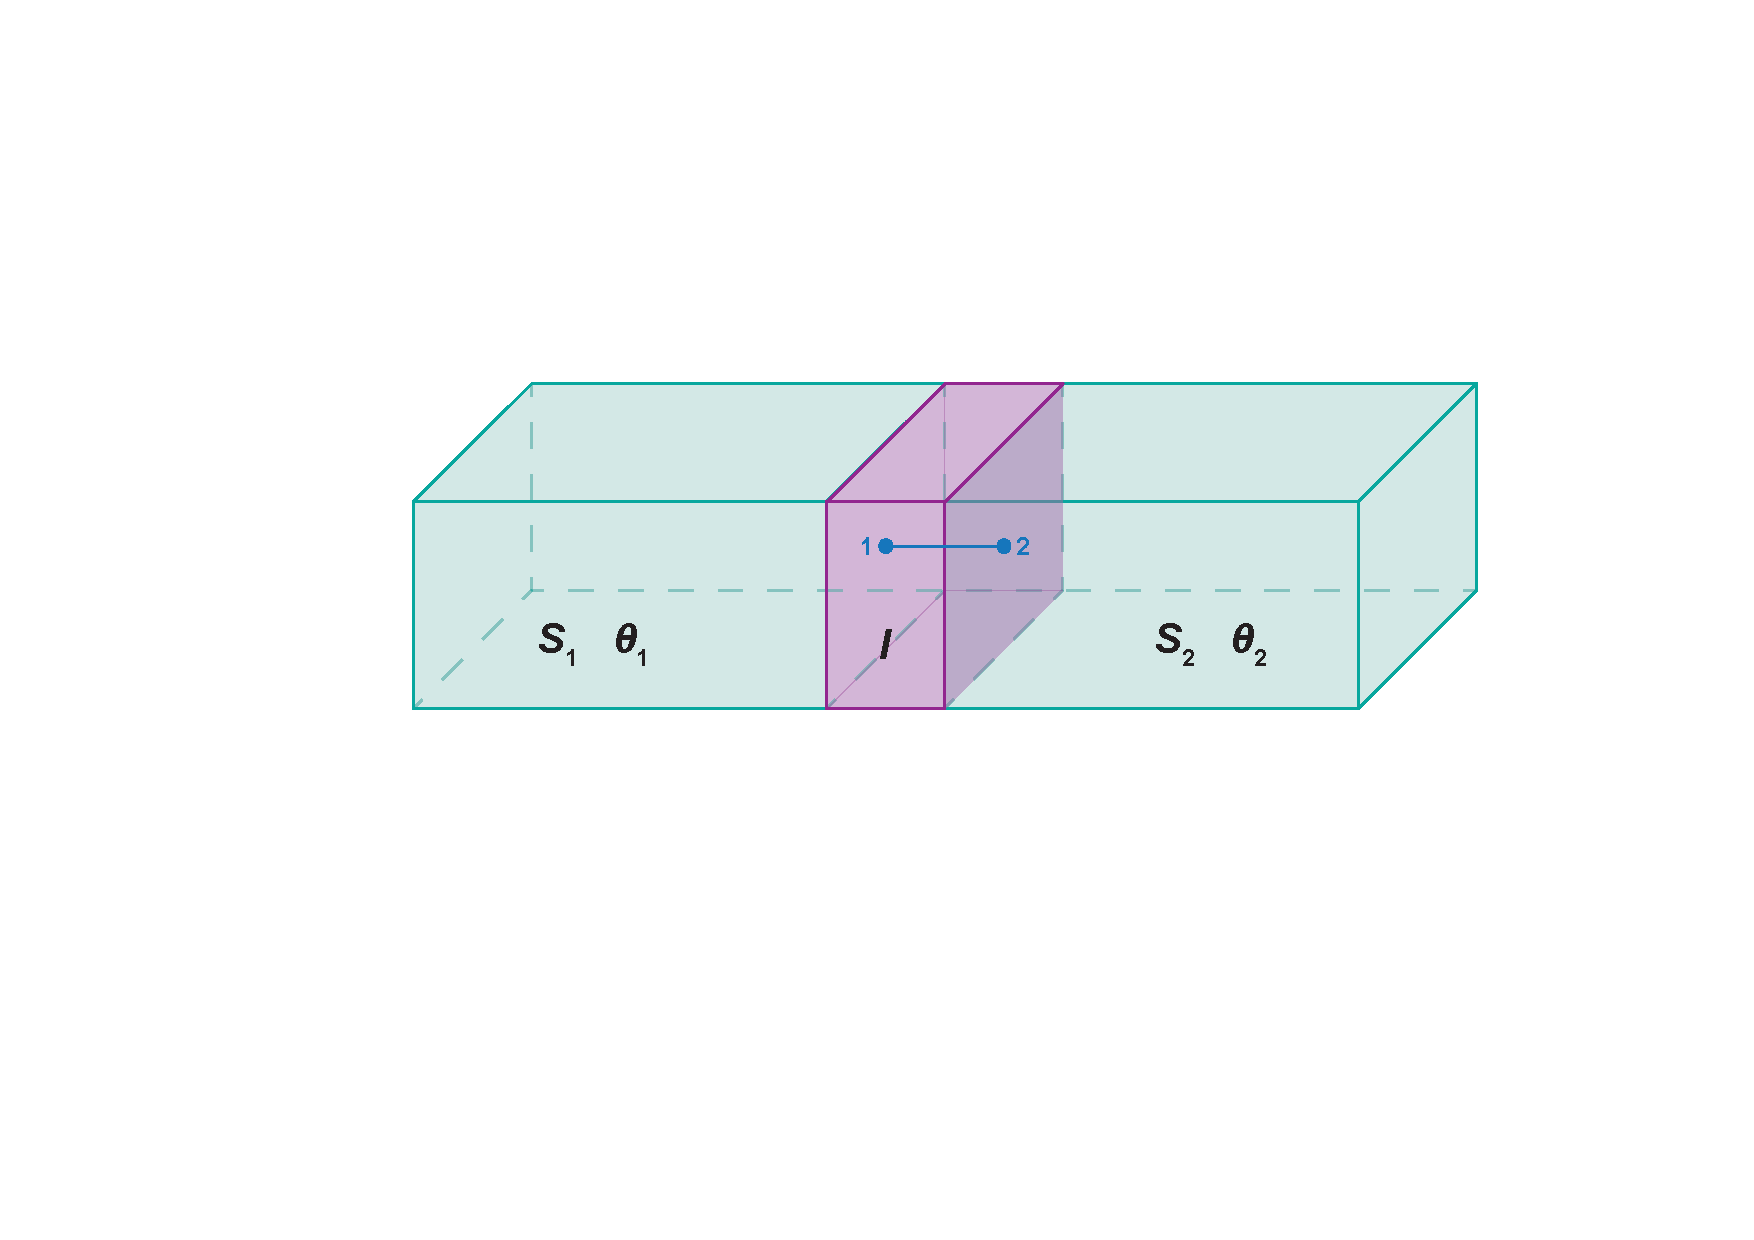
\includegraphics[width=\textwidth]{../Figures/jj_schematic}
        
\subsection{Josephson effect}

%Der Stromfluss impliziert das Tunneln von Cooper-Paaren, da bei diesen Temperaturen Niob überwiegend supraleitend ist  (${T_\mathrm{c}} = \qty{9.3}{\kelvin}$). Da die Tunnelwahrscheinlichkeit eines einzelnen Elektrons näherungsweise \textit{p} = \num{e-4} beträgt, ist bei einem Cooper-Paar bestehend aus zwei Elektronen von einer wesentlich geringeren Wahrscheinlichkeit auszugehen. Josephson sagte jedoch voraus, dass das Tunnelverhalten von Cooper-Paaren und einzelnen Leitungselektronen das gleiche sein muss. Begründet wird dies über das sogenannte \textit{Makroskopische Quantenmodell}, welches im Jahre 1953 von Fritz London formuliert wurde. \\
%Hierbei liegt das Hauptaugenmerk auf der quantenmechanischen Phase $\theta$. Zum einen sind die Abstände zwischen beiden Elektronen eines Cooper-Paares einige nm und damit erheblich größer als der Abstand der Cooper-Paare untereinander, wodurch die Wellenfunktionen stark überlappen. Zum anderen unterliegen Cooper-Paare aufgrund ihres Gesamtspins von 0 der Bose-Einstein Statistik. Somit teilen sich alle Cooper-Paare den gleichen Grundzustand und als Konsequenz sind auch die Energien bzw. Zeitentwicklungen der Phasen gleich. Diese beiden Effekte führen zu dem sogenannten \textit{phase-lock}. Die Phasen benachbarter Paare gleichen sich derart an, dass diese quantenmechanische Eigenschaft nun auf makroskopischer Skala gilt. Dies hat eine makroskopische Wellenfunktion 

The flow of current implies the tunneling of Cooper pairs, as niobium is predominantly superconducting at these temperatures ($T_\mathrm{c} = \qty{9.3}{\kelvin}$). Since the tunneling probability of an individual electron is approximately $p = \num{e-4}$, a much lower probability is to be expected for a Cooper pair consisting of two electrons. However, Josephson predicted that the tunneling behavior of Cooper pairs and individual conduction electrons must be the same. This is justified by the so-called \textit{Macroscopic Quantum Model}, formulated in 1953 by Fritz London.

The main focus here lies on the quantum mechanical phase $\theta$. On one hand, the distance between both electrons in a Cooper pair is approximately 10 to \qty{1000}{\nm} which is significantly larger than the spacing between Cooper pairs, resulting in strongly overlapping wave functions. On the other hand, Cooper pairs have to obey Bose-Einstein statistics due to their total spin of 0. Thus, all Cooper pairs share the same ground state, and as a consequence, the energies and temporal evolutions of the phases are equal. These two effects lead to what is known as \textit{phase-lock}. The phases of neighboring pairs synchronize such that this quantum mechanical property now holds on a macroscopic scale. This gives rise to a macroscopic wave function

\begin{equation}
\Psi(\textbf{r},t) = \Psi_0(\textbf{r},t)e^{i\theta(\textbf{r},t)} \ \ ,
\end{equation}

which describes all charge carriers of the superconductor. As a result of sharing the same phase, both electrons of a Cooper pair consequently possess the same tunneling probability as an individual electron, enabling the supercurrent. This coherence phenomenon is referred to as the \textit{Josephson effect} \cite{Josephson1962}. Another significant consequence of the macroscopic quantum model is flux quantization. Together with the Josephson effect, this forms the basis for Josephson junctions and their applications. 
%zur Folge, welche alle Ladungsträger des Supraleiters beschreibt. Beide Elektronen eines Cooper-Paares besitzen folglich aufgrund der geteilten Phase dieselbe Tunnelwahrscheinlichkeit wie ein einzelnes Elektron und der Suprastrom wird ermöglicht. 
%Dieses Kohärenzphänomen wird auch als \textit{Josephson-Effekt} bezeichnet.
%Eine weitere folgenreiche Konsequenz des makroskopischen Quantenmodells ist die Flussquantisierung. Diese stellt zusammen  mit dem Josephson-Effekt die Grundlage für Josephson-Kontakte und deren Anwendungen dar. \\ 

%Die Flussquantisierung wird über das Einfangen eines externen magnetischen Flusses in einem supraleitendem Zylinder hergeleitet. Die Wellenfunktion muss hier nach Umrunden des Zylinders aufgrund von $e^{i\theta}=e^{i\theta + 2\pi n}$ unverändert bleiben. Dies hat zur Folge, dass nach Integrieren entlang der stromfreien Mitte der Zylinderwand folgende Gleichung für den eingefangenen Fluss gilt

Flux quantization is derived through the capture of an external magnetic flux within a superconducting cylinder. The wave function must remain unchanged after circumnavigating the cylinder due to $e^{i\theta} = e^{i\theta + 2\pi n}$. As a result, upon integrating along the current-free center of the cylinder wall, the following equation holds for the captured flux

\begin{equation}
\Phi = \frac{h}{q_\mathrm{s}}n = \frac{h}{2e}n \equiv \Phi_0n \ \ .
\end{equation}

%Hierbei ist $n\in\mathbb{Z}$ und \unit{\fq} = \qty{2.07d-15}{\tesla\metre\squared} das sogenannte magnetische Flussquant. Der eingefangene Fluss ist damit quantisiert, was allein aus der makroskopischen Natur der Phase resultiert. Diese Größe spielt eine entscheidende Rolle bei der theoretischen Beschreibung von Josephson-Kontakten. \\

Here, $n\in\mathbb{Z}$ and \unit{\fq} = \qty{2.07e-15}{\tesla\metre\squared} \cite{CODATA2018} represents the so-called magnetic flux quantum. The captured flux is thus quantized, a consequence solely arising from the macroscopic nature of the phase. This quantity plays a crucial role in the theoretical description of Josephson junctions.

%Das Strom- und Spannungsverhalten in einem SIS-Kontakt wird über die \textit{Josephson-Gleichungen} beschrieben. Entscheidend ist hierbei ein zum eingespeisten Strom \textit{I} linear proportionaler kritischer Strom \textit{$I_\mathrm{c}$}, welcher den Grenzfall zweier Betriebsmodi bildet. \textit{I} oszilliert zudem aufgrund der makroskopischen Natur der Phase mit der eichinvarianten Phasendifferenz $\varphi$, woraus die \textbf{1. Josephson-Gleichung}

The current and voltage behavior in a SIS junction is described by the \textit{Josephson equations}. Crucial to this description is a critical current \textit{$I_\mathrm{c}$} that is linearly proportional to the applied current \textit{I}, which marks the boundary between two operational modes. Additionally, due to the macroscopic nature of the phase, \textit{I} oscillates with the gauge-invariant phase difference $\varphi$, leading to the \textbf{first Josephson equation} \cite{Josephson1965}

%Ist nämlich der eingespeiste Strom \textit{I} kleiner als \textit{$I_\mathrm{c}$}, so wird der gesamte Strom von Cooper-Paaren getragen und hängt linear von \textit{$I_\mathrm{c}$} ab. Zudem oszilliert aufgrund der makroskopischen Natur der Phase dieser mit der eichinvarianten Phasendifferenz $\varphi$, sodass gilt

 

\begin{equation}
\label{1.JE}
I_\mathrm{s} = I_\mathrm{c}\sin(\varphi) \ \ .
\end{equation}

%resultiert. $I_\mathrm{c}$ ist dabei proportional zur Kopplungsstärke $\kappa$, welche den Überlapp beider Wellenfunktionen $\Psi_1$ und $\Psi_2$ in der Isolationsschicht beschreibt. Es gilt

$I_\mathrm{c}$ is proportional to the coupling strength $\kappa$, which describes the overlap of the wave functions $\Psi_1$ and $\Psi_2$ within the insulating layer. The relationship is given by

\begin{equation}
I_\mathrm{c} = \frac{4e\kappa V n_\mathrm{s}}{\hbar} \ \ ,
\end{equation}

%wobei \textit{V} das Volumen der Supraleiterelektrode und \textit{e} die Elektronenladung bezeichnet. Es wurde zudem angenommen, dass die Cooper-Paardichte $n_\mathrm{s}$ der beiden Supraleiter $S_1$ und $S_2$ identisch ist, d.h. $n_{\mathrm{s}1} = n_{\mathrm{s}2} = n_\mathrm{s}$. \\
%Die eichinvariante Phasendifferenz bezieht sich auf die Phasen $\theta_1$ und $\theta_2$ der jeweiligen Elektroden an der Grenze zur Isolationsschicht (Position 1 und 2, siehe Abb. ?). Unter Berücksichtigung von möglichen externen elektromagnetischen Feldern innerhalb der Barriere erhält man mit dem Vektorpotential \textbf{A} die allgemeine Form

where \textit{V} represents the volume of the superconducting electrode and \textit{e} denotes the elementary charge of an electron. It was assumed that the Cooper pair density $n_\mathrm{s}$ of the two superconductors $S_1$ and $S_2$ is identical, meaning $n_{\mathrm{s}1} = n_{\mathrm{s}2} = n_\mathrm{s}$.

The gauge-invariant phase difference refers to the phases $\theta_1$ and $\theta_2$ of the respective electrodes at the boundary of the insulating layer (positions 1 and 2, see figure \ref{abb:fig:JJschem}). Taking into account possible external electromagnetic fields within the barrier, the general form using the vector potential \textbf{A} is given by \cite{Gross2016}

\begin{equation}
\label{EichInv_Phase}
\varphi = \theta_2(\textbf{r},t) - \theta_1(\textbf{r},t) - \frac{2\pi}{\Phi_0}\int_{1}^{2}\textbf{A}(\textbf{r},t)\cdot \mathrm{d}\textbf{l} \ \ .
\end{equation}

%Unter Annahme einer konstanten Dichte des Suprastroms $J_\mathrm{s}$ entlang des Kontakts erhält man durch bilden der zeitlichen Ableitung von Gleichung \eqref{EichInv_Phase} die \textbf{2. Josephson-Gleichung}

Assuming a constant supercurrent density $J_\mathrm{s}$ across the junction, taking the time derivative of equation \eqref{EichInv_Phase} yields the \textbf{second Josephson equation} \cite{Josephson1965}

\begin{equation}
\label{2.JE}
\frac{\partial\varphi}{\partial t} = \frac{2\pi}{\Phi_0}V \ \ .
\end{equation}

%Der erste Betriebsmodus beschreibt den Fall für $I<I_\mathrm{c}$. Hier wird der gesamte eingespeiste Strom von Cooper-Paaren getragen, sodass $I=I_\mathrm{s}=\mathrm{const}$. $\varphi$ ist folglich auch zeitlich konstant, womit gemäß Gleichung \eqref{2.JE} $U=0$ gilt. Dieser spannungsfreie Zustand wird auch als \textit{Josephson-Gleichstromeffekt} bezeichnet. \\
%Für $I>I_\mathrm{c}$ fangen jedoch Cooper-Paare an aufzubrechen und ein Teil des Stroms wird von Quasiteilchen getragen, welcher folglich zu einem Spannungsabfall führt. Laut der 2. Josephson-Gleichung wird die Phase $\varphi$ zeitabhängig, sodass nach Integrieren 

%\begin{equation}
%\label{phi(t)}
%\varphi = \frac{2\pi}{\Phi_0}Ut + \varphi_0 = w_\mathrm{J}t + \varphi_0 \ \ \  \mathrm{mit} \ \ \ w_\mathrm{J} = \frac{2\pi}{\Phi_0}U
%\end{equation}

%folgt. Demnach oszilliert der Strom $I_\mathrm{s}$ nach Einsetzen von Gleichung \eqref{phi(t)} in Gleichung \eqref{1.JE} mit der \textit{Josephson-Frequenz} $f_\mathrm{J} = \frac{w_\mathrm{J}}{2\pi U} = \frac{1}{\Phi_0} \approx \SI{483.6}{\MHz\per\uV}$. Entsprechend wird dieses Phänomen  \textit{Josephson-Wechselstromeffekt} genannt. 

The first operating mode describes the case for $I<I_\mathrm{c}$. Here, the entire injected current is carried by Cooper pairs, so $I=I_\mathrm{s}=\mathrm{const}$. As a result, $\varphi$ is temporally constant, which, according to equation \eqref{2.JE}, leads to $V=0$. This voltage-free state is known as the \textit{dc Josephson effect}.

For $I>I_\mathrm{c}$ however, Cooper pairs begin to break up such that a portion of the current needs to be carried by quasiparticles, which will then lead to a voltage drop \textit{V}. According to the second Josephson equation, the phase $\varphi$ becomes time dependent, and after integration one obtains

\begin{equation}
\label{phi(t)}
\varphi = \frac{2\pi}{\Phi_0}Vt + \varphi_0 = w_\mathrm{J}t + \varphi_0 \ \ \ \mathrm{with} \ \ \ w_\mathrm{J} = \frac{2\pi}{\Phi_0}V \ \ .
\end{equation}

Thus, the current $I_\mathrm{s}$ oscillates after inserting equation \eqref{phi(t)} into equation \eqref{1.JE} with the \textit{Josephson frequency} $\frac{f_\mathrm{J}}{V} = \frac{w_\mathrm{J}}{2\pi V} = \frac{1}{\Phi_0} \approx \SI{483.6}{\MHz\per\uV}$. Accordingly, this phenomenon is referred to as the \textit{ac Josephson effect}.



\subsection{Josephson Junctions in a Magnetic Field}

\Blindtext

\subsection{RCSJ Model}

\section{dc-SQUIDs}

\blindtext[3]

\subsection{Voltage State}

\subsection{Noise}

\subsection{Operation of a dc-SQUID}


\section{dc-SQUID Resonances}

\subsection{Parasitic Resonances}

\subsection{Damping Methods}


